% =====================================================================
%  Báo cáo: So sánh feature extractor cho tìm kiếm ký tự Sino-Nôm
%
%  BIÊN DỊCH (bắt buộc XeLaTeX hoặc LuaLaTeX — KHÔNG dùng pdflatex,
%  vì tài liệu nhúng chữ Hán-Nôm ngoài BMP):
%
%      cd comparing-character-glyph-images-Sino-N-m
%      latexmk -xelatex -cd report/report.tex
%      # hoặc: cd report && xelatex report.tex   (chạy 2 lần, lấy mục lục)
%
%  Font chữ Hán-Nôm lấy từ ./fonts (tải bằng `bash download_fonts.sh`).
%  Đường dẫn font (../fonts/) và ảnh (figs/) là TƯƠNG ĐỐI so với thư mục
%  report/, nên phải biên dịch từ trong report/ — tuỳ chọn -cd của latexmk
%  tự chuyển vào đó.
% =====================================================================
\documentclass[11pt,a4paper]{article}

\usepackage{fontspec}
\usepackage{geometry}
\geometry{margin=2.5cm}
\usepackage{booktabs}
\usepackage{array}
\usepackage{graphicx}
\usepackage{caption}
\usepackage{xcolor}
\usepackage{amssymb}
\usepackage[hidelinks]{hyperref}

% --- Font chữ Latinh: TeX Gyre Termes phủ đủ dấu tiếng Việt ---------
% Ligatures=TeX để "---" ra gạch dài; CỐ TÌNH không bật cho font mono,
% nếu không thì các cờ dòng lệnh như --normalize sẽ bị nối thành gạch ngang.
\setmainfont{TeX Gyre Termes}[Ligatures=TeX]
\setsansfont{TeX Gyre Heros}[Ligatures=TeX]
\setmonofont{TeX Gyre Cursor}[Scale=0.92]

% --- Font chữ Hán-Nôm -----------------------------------------------
% BabelStone Han phủ gần hết ký tự dùng trong báo cáo, kể cả Ext-B.
% Ba ký tự 𣦰 𤟂 𦝊 không có trong BabelStone -> dùng \nomb (HanaMinB).
\newfontfamily\nomfont{BabelStoneHan.ttf}[Path=../fonts/]
\newfontfamily\nomfontb{HanaMinB.otf}[Path=../fonts/]
\newcommand{\nom}[1]{{\nomfont #1}}
\newcommand{\nomb}[1]{{\nomfontb #1}}

\newcommand{\code}[1]{\texttt{#1}}
\newcommand{\up}{$\uparrow$}
\newcommand{\dn}{$\downarrow$}

\title{\textbf{So sánh Feature Extractor cho bài toán\\
tìm kiếm ký tự Sino-Nôm tương đồng}}
\author{Báo cáo phần việc: thay ResNet18 bằng backend họ Transformer\\
và đo hiệu quả so với baseline}
\date{}

\begin{document}
\maketitle

\begin{abstract}
\noindent
Báo cáo so sánh sáu feature extractor trên corpus 26.044 ảnh glyph Sino-Nôm.
\code{chinese-clip-large} hơn baseline ResNet18 \textbf{2,31 lần} ở \code{radical@k}, và việc
scale tiếp lên ViT-H làm kết quả \emph{giảm} 4,0\% --- mô hình to hơn không đồng nghĩa tốt hơn.
Nhưng phát hiện quan trọng hơn nằm ở chỗ khác: khi đo trên \textbf{59 ảnh scan thật} thay vì dùng
nhãn yếu, \code{hit@1} chỉ đạt \textbf{0,0847}. Nguyên nhân không phải mô hình kém mà là
\textbf{lệch phân phối}: query là chữ viết tay/hành thư còn corpus là khải thư in bằng font.
Bài toán thu hẹp theo âm Quốc Ngữ (Phần 2) thì dùng được ngay --- 0,4746 --- nhưng cỡ mẫu
$n = 59$ khiến mọi so sánh dưới 15 điểm nằm trong khoảng nhiễu, kể cả khoảng cách giữa embedding
và histogram. Báo cáo ghi lại cả các kết quả âm và các lần tự sửa sai, vì chúng ràng buộc kết luận
chặt hơn các con số thuận lợi.
\end{abstract}

\tableofcontents
\bigskip
\hrule

% =====================================================================
\section{Bài toán và câu hỏi cần trả lời}

Baseline của đồ án dùng ResNet18 (CNN, pretrain ImageNet) để trích đặc trưng ảnh glyph, rồi tìm
top-$K$ lân cận bằng Faiss. Hai câu hỏi:

\begin{enumerate}
  \item ResNet18 baseline yếu tới mức nào, và \textbf{nguyên nhân nằm ở đâu}?
  \item Feature extractor họ Transformer có thật sự tốt hơn không, và \textbf{hơn bao nhiêu}?
\end{enumerate}

Hệ thống có hai phần việc khác nhau, và báo cáo giữ chúng tách bạch vì độ khó chênh nhau nhiều bậc:

\begin{description}
  \item[Phần 1] Cho một ảnh, tìm ký tự giống nhất trong \textbf{toàn bộ 26.044} ký tự corpus.
  \item[Phần 2] Cho một ảnh \emph{và} âm Quốc Ngữ của nó, xếp hạng trong nhóm ký tự cùng âm ---
        trung vị 7 ứng viên, nhiều nhất 97 (âm ``tư'').
\end{description}

% =====================================================================
\section{Thiết lập thí nghiệm}

\begin{table}[h]
\centering
\begin{tabular}{ll}
\toprule
Hạng mục & Giá trị \\
\midrule
Corpus & 26.044 ảnh glyph (trên 31.208 dòng bảng; 5.164 dòng không có ảnh) \\
top-$K$ & 20 \\
Chỉ mục & Faiss \code{IndexFlatIP} trên vector chuẩn hoá L2 ($\Rightarrow$ cosine) \\
Phần cứng & NVIDIA H100 80\,GB (dùng chung với 4 engine vLLM), 16 nhân CPU \\
Môi trường & Python 3.10.12, torch 2.6.0+cu124, transformers 4.57.6 \\
Tính tất định & \code{set\_deterministic(seed=42)}, tắt cudnn benchmark \\
\bottomrule
\end{tabular}
\caption{Thiết lập chung.}
\end{table}

\begin{table}[h]
\centering
\small
\begin{tabular}{llrll}
\toprule
backend & mô hình & chiều & dtype & vai trò \\
\midrule
\code{resnet18} & ResNet18 ImageNet & 512 & fp32 & baseline gốc, giữ nguyên từng dòng \\
\code{resnet18-gray} & ResNet18, \code{conv1} từ trọng số pretrained & 512 & fp32 & biến thể kiểm chứng giả thuyết \\
\code{chinese-clip} & OFA-Sys/chinese-clip-vit-base-patch16 & 512 & fp32 & ViT-B/16 \\
\code{chinese-clip-large} & OFA-Sys/chinese-clip-vit-large-patch14 & 768 & fp16 & ViT-L/14 \\
\code{chinese-clip-huge} & OFA-Sys/chinese-clip-vit-huge-patch14 & 1024 & fp16 & ViT-H/14 \\
\code{dinov2} & facebook/dinov2-base & 1536 & fp32 & ViT tự giám sát, CLS $\oplus$ mean patch \\
\bottomrule
\end{tabular}
\caption{Sáu backend. Ba dòng \code{chinese-clip*} cùng một họ và cùng dữ liệu pretrain, nên chuỗi
base $\to$ large $\to$ huge cô lập được đúng ảnh hưởng của việc scale.}
\end{table}

\subsection{Hai thủ thuật bộ nhớ, và việc kiểm chứng fp16}

GPU chỉ còn khoảng 3,05\,GB trống (4 engine vLLM chiếm phần còn lại) trong khi ViT-H/14 fp32 cần
$\sim$3,8\,GB. Hai thay đổi giúp nó vừa: (1) \textbf{bỏ tháp text trước khi đưa lên GPU} ---
\code{get\_image\_features} chỉ dùng \code{vision\_model} và \code{visual\_projection}, nhưng
\code{ChineseCLIPModel} nạp thêm cả một RoBERTa hoàn chỉnh, riêng với ViT-H là $\sim$1,3\,GB nạp
lên rồi không bao giờ dùng; (2) \textbf{fp16}.

fp16 được \emph{kiểm chứng} chứ không giả định. So trên chính \code{chinese-clip} base (đã có số
fp32): $\cos(\text{fp32}, \text{fp16}) \geq 0{,}99999$ và trùng \textbf{99,31\%} danh sách top-20.
Nên số của các model fp16 vẫn so sánh công bằng được với các model fp32.

\subsection{Vì sao có \code{resnet18-gray}}

Baseline thay \code{conv1} của ResNet18 bằng một conv 1 kênh mới. Thao tác này \textbf{vứt bỏ toàn
bộ bộ lọc tầng đầu đã pretrain và thay bằng trọng số ngẫu nhiên} --- mọi tầng phía sau đang xử lý
đầu ra của một bộ dò biên ngẫu nhiên. \code{resnet18-gray} sửa đúng một dòng đó: cộng 3 kênh RGB
của bộ lọc pretrain thành 1 kênh. Đây là biến thể để kiểm chứng giả thuyết ``baseline yếu vì lỗi
\code{conv1}'' (kết quả ở mục~\ref{sec:conv1}).

% =====================================================================
\section{Phương pháp đánh giá, và giới hạn của nó}

Pipeline tìm kiếm \textbf{chỉ dùng ảnh}. Vì vậy có thể lấy các cột metadata mà pipeline không hề
đụng tới trong \code{final\_characteristics-v2.xlsx} làm nhãn yếu để chấm điểm:

\begin{table}[h]
\centering
\begin{tabular}{lll}
\toprule
chỉ số & định nghĩa & nguồn \\
\midrule
\code{radical@k} \up & tỉ lệ lân cận top-$K$ cùng bộ thủ với query & \code{RADICAL} \\
\code{stroke\_mae@k} \dn & trung bình $|$chênh lệch số nét$|$ & \code{STROKE\_NUM} \\
\code{ids\_jaccard@k} \up & Jaccard giữa các thành phần IDS & \code{SHAPE\_MORPH} \\
\bottomrule
\end{tabular}
\end{table}

\begin{quote}
\textbf{Giới hạn quan trọng.} Đây \textbf{không phải} đánh giá của con người. Chúng là các chỉ số
thay thế (proxy) rẻ tiền, tương quan với ``trông giống nhau'', đủ để \emph{xếp hạng các backend với
nhau} --- và không hơn. Mục~\ref{sec:tran} cho thấy chính các proxy này cũng có trần riêng, còn
mục~\ref{sec:that} thay chúng bằng nhãn thật.
\end{quote}

% =====================================================================
\section{Kết quả so sánh backend}

\subsection{Chất lượng (full corpus 26.044 glyph, top-$K$ = 20)}

\begin{table}[h]
\centering
\begin{tabular}{lrrrr}
\toprule
backend & chiều & \code{radical@k} \up & \code{stroke\_mae@k} \dn & \code{ids\_jaccard@k} \up \\
\midrule
\code{resnet18} (baseline) & 512 & 0,2316 & 2,8942 & 0,1031 \\
\code{resnet18-gray} & 512 & 0,2202 & 2,5658 & 0,1020 \\
\code{chinese-clip} & 512 & 0,4843 & 2,6296 & 0,1997 \\
\textbf{\code{chinese-clip-large}} & 768 & \textbf{0,5361} & 2,6992 & 0,2113 \\
\code{chinese-clip-huge} & 1024 & 0,5147 & 2,6547 & \textbf{0,2144} \\
\code{dinov2} & 1536 & 0,3081 & \textbf{2,3397} & 0,1251 \\
\bottomrule
\end{tabular}
\caption{So với baseline, \code{chinese-clip-large} đạt \code{radical@k} \textbf{gấp 2,31 lần} và
\code{ids\_jaccard} \textbf{gấp 2,05 lần}.}
\end{table}

\subsection{Tốc độ}

\begin{table}[h]
\centering
\begin{tabular}{lrrr}
\toprule
backend & CPU 16 nhân & H100 & full 26k trên GPU \\
\midrule
\code{resnet18} & $\sim$347 img/s & 3.950 img/s & 6,6 s \\
\code{resnet18-gray} & $\sim$403 img/s & 3.937 img/s & 6,6 s \\
\code{chinese-clip} & $\sim$5--9 img/s & 358 img/s & 73 s \\
\code{chinese-clip-large} & chưa đo & 354 img/s & 74 s \\
\code{chinese-clip-huge} & chưa đo & 283 img/s & 92 s \\
\code{dinov2} & $\sim$7 img/s & 306 img/s & 85 s \\
\bottomrule
\end{tabular}
\end{table}

\code{chinese-clip-large} gấp đôi tham số so với base nhưng \textbf{gần như không tốn thêm thời
gian} (354 so với 358 img/s) --- fp16 bù lại đúng phần chi phí tăng thêm. Chuyển sang GPU giúp
backend ViT nhanh gấp $\sim$45 lần, đủ để chạy full corpus thay vì phải dùng \code{--limit}.

\begin{quote}
Số tốc độ chỉ mang tính tham khảo ($\pm$10\%): H100 dùng chung với 4 engine vLLM, tải thay đổi
theo thời gian. Ngược lại, các chỉ số chất lượng là tất định và lặp lại chính xác.
\end{quote}

\subsection{Mức đồng thuận giữa các backend}

Số lân cận trùng nhau trung bình trên top-20 chỉ đạt \textbf{7,6--12,9\%}: cặp gần nhau nhất
(\code{chinese-clip} $\leftrightarrow$ \code{dinov2}) trùng 2,57/20 = 12,9\%; cặp xa nhất
(\code{resnet18} $\leftrightarrow$ \code{dinov2}) trùng 1,52/20 = 7,6\%.

Hai hệ quả: (1) các chỉ số proxy đang thực sự \emph{phân biệt được} các backend chứ không đo cùng
một thứ; (2) đánh giá bằng người sẽ mang tính \emph{quyết định} chứ không phải chỉ để xác nhận ---
vì các mô hình không hội tụ về một đáp án chung nào cả.

% =====================================================================
\section{Phân tích}

\subsection{Scale có lợi, nhưng bão hoà rồi đảo chiều}

Đây là phát hiện đáng giá nhất từ việc thêm hai model lớn:

\begin{center}
\begin{tabular}{lrr}
\toprule
bước scale & \code{radical@k} & thay đổi \\
\midrule
base $\to$ large & $0{,}4843 \to 0{,}5361$ & \textbf{+10,7\%} \\
large $\to$ huge & $0{,}5361 \to 0{,}5147$ & \textbf{$-$4,0\%} \\
\bottomrule
\end{tabular}
\end{center}

\code{chinese-clip-huge} nhiều tham số hơn đáng kể, tốn thêm 33\% số chiều và 20\% thời gian,
nhưng lại \emph{kém hơn}. Hệ quả thực tế: \textbf{\code{chinese-clip-large} là điểm ngọt}, và nếu
ai đề xuất thử tiếp ViT-G thì đây là bằng chứng cho thấy nhiều khả năng không đáng.

Giả thuyết cho việc bão hoà (\emph{chưa kiểm chứng}): các model CLIP lớn được tối ưu cho ảnh tự
nhiên đa dạng, trong khi glyph là ảnh gần nhị phân, một kênh, cấu trúc rất hẹp. Khi mô hình đủ lớn
để bắt cấu trúc nét, phần dung lượng tăng thêm dùng cho những đặc trưng bài toán này không cần.

\subsection{DINOv2 bổ sung cho họ CLIP, không đơn thuần là kém hơn}

Không có người thắng tuyệt đối. Mọi backend \code{chinese-clip*} thắng ở \code{radical@k} và
\code{ids\_jaccard@k} --- các tín hiệu \emph{cấu trúc}. Còn \code{dinov2} thắng ở
\code{stroke\_mae@k} (2,3397, tốt nhất trong sáu) --- bám sát \emph{mật độ nét} hơn.

Kiểm chứng định tính khớp với số liệu. Với query bộ \nom{犭} (\nomb{𤟂}), \code{resnet18} trả
\nom{猜 指 𢯡 褃 棈} (lẫn lộn \nom{犭/扌/礻/米}) còn \code{chinese-clip} trả \nom{猎 狺 猜 獍 獖}
(gần như toàn bộ \nom{犭}). Ngược lại, với query bộ \nom{月} (\nomb{𦝊}) thì \code{dinov2} trả
\nom{腿 脙}\nomb{ 𦟂 }\nom{胣 膔} (gần như toàn bộ \nom{月}) trong khi \code{chinese-clip} lệch sang bộ \nom{辶}.

Kết hợp với mức đồng thuận 12,9\%, đây là bằng chứng cho thấy hai họ nhìn chữ theo hai cách khác
nhau --- \textbf{ensemble hoặc rerank là bước tiếp theo hợp lý}.

\subsection{Giả thuyết lỗi \code{conv1} \emph{không} đúng}
\label{sec:conv1}

\code{resnet18-gray} sửa đúng lỗi khởi tạo ngẫu nhiên. Kết quả: \code{stroke\_mae@k} cải thiện
($2{,}8942 \to 2{,}5658$, tốt hơn 11,3\%), nhưng \code{radical@k} \emph{tệ đi}
($0{,}2316 \to 0{,}2202$) và \code{ids\_jaccard@k} gần như không đổi.

Vậy lỗi \code{conv1} \textbf{không phải} nguyên nhân chính khiến baseline yếu. Đây là một
\textbf{kết quả âm}, và nó có giá trị: nó loại bỏ một giả thuyết rẻ tiền, cho thấy khoảng cách chất
lượng đến từ bản thân kiến trúc/prior của mô hình chứ không phải một dòng code hỏng. Chính điều này
biện minh cho việc chuyển hẳn sang backend ViT.

% =====================================================================
\section{\code{radical@k} có thật sự ``bão hoà ở 0,5''?}
\label{sec:tran}

Ba giả thuyết được nêu cho việc \code{radical@k} dừng quanh 0,5. Mục này kiểm chứng từng cái bằng
số đo (\code{analyze\_metric\_ceiling.py}).

\subsection{Giả thuyết ``tập top-$k$ bị thiếu ứng viên'': bị bác bỏ}

Nếu corpus không đủ ký tự cùng bộ thủ để lấp đầy 20 chỗ thì \code{radical@20} không thể đạt 1,0.
Với query có bộ thủ $r$ thuộc nhóm $c$ phần tử, trần của riêng query đó là $\min(c-1,k)/k$. Tính ra:
trần lý thuyết của \code{radical@20} là \textbf{0,9862}, và chỉ \textbf{888/26.035 query (3\%)} bị
chạm trần. Kích thước tập top-$k$ không phải nguyên nhân.

Bằng chứng thứ hai, mạnh hơn: nghẽn nằm ngay ở láng giềng \emph{gần nhất}.

\begin{table}[h]
\centering
\small
\begin{tabular}{lrrrrrrrr}
\toprule
backend & @1 & @2 & @3 & @5 & @10 & @20 & @50 & @100 \\
\midrule
\code{chinese-clip} & 0,5825 & 0,5628 & 0,5508 & 0,5347 & 0,5121 & 0,4843 & 0,4398 & 0,3989 \\
\textbf{\code{chinese-clip-large}} & \textbf{0,6331} & 0,6124 & 0,5994 & 0,5833 & 0,5606 & \textbf{0,5361} & 0,4965 & 0,4565 \\
\code{chinese-clip-huge} & 0,6081 & 0,5888 & 0,5744 & 0,5588 & 0,5392 & 0,5147 & 0,4745 & 0,4350 \\
\code{dinov2} & 0,4674 & 0,4417 & 0,4238 & 0,3963 & 0,3549 & 0,3081 & 0,2461 & 0,2019 \\
\code{resnet18} & 0,3851 & 0,3532 & 0,3349 & 0,3072 & 0,2697 & 0,2316 & 0,1818 & 0,1477 \\
\code{resnet18-gray} & 0,3836 & 0,3519 & 0,3290 & 0,2998 & 0,2598 & 0,2202 & 0,1716 & 0,1401 \\
\bottomrule
\end{tabular}
\caption{\code{radical@k} theo $k$. Đường cong xuống rất thoải, tức đây \emph{không} phải hiện
tượng ``loãng dần vì lấy quá nhiều''.}
\end{table}

Ngay cả ứng viên số 1 cũng chỉ cùng bộ thủ 63\% số lần. Có nới $k$ xuống 1 thì con số cũng chỉ lên
0,6331.

\subsection{Trần \emph{thực tế} là 0,73 chứ không phải 0,99 --- nhãn mới là chỗ nghẽn}

Trần 0,9862 giả định tồn tại một bộ rank hoàn hảo. Nhưng \code{RADICAL} \textbf{không phải nhãn thị
giác thuần tuý}:

\begin{itemize}
  \item Bộ thủ chỉ \emph{xuất hiện thật} trong phân rã IDS của chính chữ đó ở \textbf{56,7\%} số ký
        tự. Với 43,3\% còn lại, bộ thủ là quy ước tra từ điển, \textbf{không nhìn thấy được từ hình
        chữ}.
  \item Cặp cùng bộ thủ có IDS-Jaccard trung bình 0,2571 (khác bộ thủ: 0,0009). Tín hiệu có thật
        nhưng yếu --- cùng bộ thủ \emph{không} kéo theo trông giống nhau.
\end{itemize}

Để định lượng, dựng một \textbf{oracle} xếp hạng bằng Jaccard trên thành phần IDS \emph{thật} (lấy
thẳng từ \code{SHAPE\_MORPH}) --- tức một bộ rank ``biết trước cấu trúc chữ'', tốt hơn bất kỳ mô
hình thị giác nào có thể suy ra từ ảnh.

\begin{center}
\begin{tabular}{lr}
\toprule
bộ xếp hạng & \code{radical@20} \\
\midrule
ngẫu nhiên & 0,0220 \\
\code{resnet18} (baseline) & 0,2316 \\
\code{chinese-clip-large} & \textbf{0,5361} \\
\textbf{oracle IDS-Jaccard} (biết trước cấu trúc) & \textbf{0,7338} \\
trần lý thuyết & 0,9862 \\
\bottomrule
\end{tabular}
\end{center}

\textbf{\code{chinese-clip-large} đang đạt 73\% của oracle} ($0{,}5361/0{,}7338$) và
\textbf{24,4$\times$ mức ngẫu nhiên}. Khoảng trống còn lại tới oracle là \textbf{+37\% tương đối},
không phải ``gấp đôi''. Nói cách khác: 0,5 trông như bão hoà chỉ vì đang so với 1,0; so với trần
đúng của bài toán thì nó nằm ở khoảng ba phần tư quãng đường.

\subsection{Giả thuyết ``pretrain sai domain'': đúng, và có bằng chứng gián tiếp}

Không đo trực tiếp được, nhưng ba dữ kiện cùng chỉ một hướng:

\begin{enumerate}
  \item Chinese-CLIP huấn luyện contrastive ảnh--văn bản trên ảnh web tiếng Trung; đặc trưng của nó
        ở tầng \emph{ngữ nghĩa cảnh vật}, không phải tầng \emph{nét bút}. Ở đây tháp text đã bị xoá,
        chỉ còn tháp ảnh --- nó chưa từng được dạy rằng ``cùng bộ thủ'' là quan hệ đáng quan tâm.
  \item \textbf{Scale bão hoà rồi quay đầu} ($-4{,}0\%$ ở bước large $\to$ huge) đúng là chữ ký của
        ``thêm dung lượng cho một mục tiêu huấn luyện sai''. Nếu chỉ thiếu năng lực biểu diễn thì
        huge đã phải tốt hơn large.
  \item \code{dinov2} (tự giám sát thuần ảnh) thắng ở \code{stroke\_mae@k} nhưng thua xa ở
        \code{radical@k}, và chỉ trùng 12,9\% top-$k$ --- chưa model nào bắt được ``cấu trúc chữ''.
\end{enumerate}

Kết luận: \textbf{finetune là đòn bẩy thật.} Kèm một cái bẫy --- nếu finetune trên nhãn
\code{RADICAL} rồi lại báo cáo \code{radical@k} thì chỉ số sẽ tăng vọt mà \emph{không chứng minh
được gì}, vì đó là đo lại tập huấn luyện. Bắt buộc phải chia held-out \emph{theo bộ thủ}, huấn
luyện trên một nhãn và đánh giá trên nhãn khác, và giữ nguyên các mốc zero-shot trong cùng bảng.

% =====================================================================
\section{Đánh giá trên ảnh scan thật --- phép đo duy nhất không phải proxy}
\label{sec:that}

Tất cả các mục trước đều dùng nhãn yếu và query là chính ảnh corpus. Mục này khác hẳn: query là
\textbf{59 ảnh scan} trong \code{test\_images/}, và \textbf{nhãn là thật}.

\subsection{Nhãn đến từ đâu}

Tên file được gõ Telex: \code{cofn.jpg} = ``còn'', \code{truwowsc.jpg} = ``trước''. Giải mã ngược
rồi tra \code{QuocNgu\_SinoNom\_Dic.xlsx} cho ra tập ký tự Sino-Nôm đúng của ảnh đó. Telex cho phép
đặt dấu thanh ngay sau nguyên âm (\code{cofn}) lẫn ở cuối từ (\code{conf}), nên bộ giải mã sinh mọi
vị trí đặt dấu rồi khớp. Kết quả: \textbf{59/59 khớp, không có trường hợp nhập nhằng}.

Trước đây con số này là 56/59, và ba ảnh bị loại vì ba lý do khác nhau --- chỉ một trong ba là lỗi
dữ liệu:

\begin{itemize}
  \item \code{phong\_1} --- \textbf{lỗi code}. \code{decode\_filenames} gọi \code{words.pop()} trên
        chính cái \code{set} đang nằm trong \code{lookup}, nên sau khi khớp \code{phong.jpg} thì
        \code{lookup["phong"]} rỗng và ảnh thứ hai của \emph{bất kỳ} từ lặp nào cũng bị âm thầm bỏ.
        Đã sửa thành \code{next(iter(words))}.
  \item \code{dau} --- gõ thiếu dấu mũ; văn bản là ``bể \textbf{dâu}'', phân biệt với
        \code{ddau.jpg} = ``đau''.
  \item \code{nguwowsi} --- gõ \code{s} (sắc) thay vì \code{f} (huyền); từ đúng là ``người''.
\end{itemize}

Hai trường hợp sau sửa bằng bảng \code{FILENAME\_FIXES} trong code thay vì đổi tên file, để
\code{test\_images/} còn khớp byte-đối-byte với zip gốc.

\subsection{Phần 1 --- tìm trên toàn bộ 26.044 ký tự}

\begin{center}
\begin{tabular}{lr}
\toprule
chỉ số & \code{chinese-clip-large} fp16 \\
\midrule
\code{hit@1} & 5/59 = \textbf{0,0847} \\
\code{hit@5} & 9/59 = 0,1525 \\
\code{hit@10} & 11/59 = 0,1864 \\
\code{hit@20} & 12/59 = 0,2034 \\
MRR & 0,1143 \\
baseline ngẫu nhiên \code{hit@1} & 0,000474 \\
\bottomrule
\end{tabular}
\end{center}

\textbf{Hơn ngẫu nhiên 179$\times$, nhưng tuyệt đối thì thấp.} Đây là con số trung thực đầu tiên của
đồ án, và nó thấp hơn hẳn những gì các chỉ số proxy gợi ý. Cần nói rõ điều này thay vì chỉ khoe
\code{radical@k}.

\subsection{Vì sao thấp: lệch phân phối, không phải model kém}

Dấu hiệu đầu tiên là \textbf{hub effect} --- top-1 lặp lại bất thường: \nom{攅} xuất hiện 6 lần,
\nom{劕/湸/旦/刟} mỗi chữ 3 lần trên các query khác nhau. Query nằm ngoài phân phối nên tất cả bị
hút về vài vector corpus. Đo trực tiếp mức lệch:

\begin{table}[h]
\centering
\begin{tabular}{lrr}
\toprule
 & \code{test\_images/} (scan) & \code{images/} (corpus) \\
\midrule
tỉ lệ điểm ảnh có mực & \textbf{0,353} & 0,184 \\
chiều cao hộp bao / khung & 0,919 & 0,800 \\
chiều rộng hộp bao / khung & 0,927 & 0,743 \\
giá trị nền & 249 (xám, nhiễu scan) & 255 (trắng tuyệt đối) \\
kích thước & 88$\times$96, 96$\times$128\ldots \textbf{không vuông} & \textbf{70$\times$70, luôn vuông} \\
\bottomrule
\end{tabular}
\end{table}

Nhưng nguyên nhân \emph{lớn nhất} chỉ nhìn bằng mắt mới thấy: \textbf{query là chữ viết tay / hành
thư, corpus là khải thư in bằng font sạch}. \code{moojt.jpg} (``một'') là \nom{沒} viết tay nét cong
mềm, trong khi 9 ứng viên corpus đều là khải thư ngay ngắn. \code{cofn.jpg} (``còn'') là \nom{群}
viết tay --- đáp án đúng \emph{có} trong corpus, và Phần 2 xếp nó hạng 2/5.

Nghĩa là thông tin cần thiết \emph{có} trong ảnh; mô hình phải bắc cầu giữa hai kiểu thư pháp, việc
mà Chinese-CLIP chưa bao giờ được dạy. Đây chính là giả thuyết ``pretrain sai domain'', nhưng lần
này quan sát được trực tiếp thay vì suy ra từ đường cong scale.

\subsection{Thử chuẩn hoá hình học: không đủ}

\code{--normalize} cắt sát nét mực, đệm vào khung vuông, đưa chữ về đúng tỉ lệ chiếm khung như corpus:

\begin{table}[h]
\centering
\begin{tabular}{lrrrrr}
\toprule
biến thể & \code{hit@1} & \code{hit@5} & \code{hit@20} & MRR & số top-1 khác nhau \\
\midrule
A. gốc & 0,0847 & 0,1525 & 0,2034 & 0,1143 & 41/59 \\
B. chuẩn hoá \textbf{query} & \textbf{0,1017} & 0,1525 & \textbf{0,2542} & \textbf{0,1286} & \textbf{48/59} \\
C. chuẩn hoá \textbf{cả hai phía} & 0,0847 & \textbf{0,1864} & 0,2203 & 0,1203 & 39/59 \\
\bottomrule
\end{tabular}
\end{table}

\begin{quote}
\textbf{Đừng đọc bảng này như một chiến thắng.} Ở $n = 59$, chênh lệch \code{hit@1} giữa A và B là
\textbf{5 ảnh so với 6 ảnh} --- đúng một ảnh, nằm gọn trong khoảng nhiễu. Ở $n = 56$ khoảng cách này
là 4 so với 6 ảnh; thêm ba ảnh đã làm nó co lại, minh hoạ đúng vì sao không được đọc bảng này theo
hướng có lợi. Điều duy nhất kết luận được là \textbf{hub effect giảm rõ} ($41 \to 48$ top-1 khác
nhau), tức chuẩn hoá có sửa được phần lệch \emph{hình học}.
\end{quote}

Phần còn lại --- khoảng cách thư pháp --- chuẩn hoá không chạm tới được. Vì vậy \code{--normalize}
\textbf{không bật mặc định}.

\subsection{Phần 2 trên scan thật --- đây mới là chỗ dùng được}

Phần 2 chỉ xếp hạng trong nhóm cùng âm nên bài toán dễ hơn nhiều bậc. Ví dụ
\code{--word còn --image test\_images/cofn.jpg}:

\begin{center}
\begin{tabular}{llll}
\toprule
 & top-1 & top-2 & top-3 \\
\midrule
embedding & \nom{存} 0,8036 & \textbf{\nom{群} 0,7994} $\leftarrow$ đúng & \nom{羣} 0,7883 \\
histogram & \nom{噲} 0,9987 & \nom{羣} 0,9984 & \nom{群} 0,9954 \\
\bottomrule
\end{tabular}
\end{center}

Chú ý điểm số histogram: cách nhau \textbf{0,003 trên toàn nhóm}, gần như không phân biệt được gì,
trong khi embedding trải từ 0,80 xuống 0,72. Trên toàn bộ 59 ảnh, hai phương pháp chỉ chọn cùng
top-1 ở \textbf{23/59 (39,0\%)}.

\subsection{Gán nhãn Phần 2, và thang tin cậy}

Chấm điểm Phần 2 cho đúng cần biết ảnh scan đó \emph{là ký tự cụ thể nào}. 59 ảnh là mười mấy câu
mở đầu \emph{Truyện Kiều}, nên ngoài so hình còn đối chiếu được với chính tả Nôm của văn bản. Quy
trình: (1) so hình là chính; (2) đối chiếu văn bản Kiều làm tiên nghiệm; (3) khi mâu thuẫn thì
\textbf{theo hình}, vì đang gán nhãn cho ảnh này chứ không cho một ấn bản --- có xảy ra thật:
``qua'' trong scan là \nom{戈} chứ không phải \nom{過}, ``năm'' là \nom{𢆥} chứ không phải \nom{年}.

\paragraph{Cột \code{confidence} tính từ đâu?} Không từ đâu cả --- đây là \textbf{đánh giá của người
đọc ảnh, không suy ra từ bất kỳ điểm số nào của mô hình}, và điều đó là cố ý. Có một phép kiểm dùng
chính cột này để lọc ra tập nhãn chắc chắn rồi chấm lại mô hình; nếu \code{confidence} lấy từ điểm
similarity thì phép kiểm ấy thành vòng tròn --- lấy mô hình chấm mô hình.

\begin{table}[h]
\centering
\begin{tabular}{llr}
\toprule
mức & tiêu chí & $n$ \\
\midrule
\code{high} & nét quyết định đọc được; mọi ứng viên còn lại khác ở \textbf{bộ thủ} hoặc \textbf{số nét thấy rõ} & 53 \\
\code{med} & còn $\geq 1$ ứng viên là \textbf{biến thể gần trùng}, chỉ khác ở chi tiết đã mờ/mất & 4 \\
\code{low} & nét quyết định \textbf{không} đọc được; chọn dựa vào văn cảnh nhiều hơn hình & 2 \\
\bottomrule
\end{tabular}
\end{table}

\paragraph{Một lỗi thiết kế phiếu đã sửa.} Hàm sinh phiếu mặc định cắt danh sách ở 24 ứng viên,
trong khi cột \code{n\_candidates} vẫn ghi tổng số thật --- phiếu tự mâu thuẫn. Bốn ảnh dính lỗi
này (\code{gia} 32/50, \code{lujc} 35/40, \code{phong} 30/35, \code{tuw} 27/97), và ở cả bốn thì
\textbf{đáp án đúng nằm ngoài phần được in}: người gán nhãn không thể chọn đúng. Nay liệt kê hết và
kèm codepoint cho từng ứng viên.

\subsection{Kết quả Phần 2 ($n = 59$)}

\begin{table}[h]
\centering
\begin{tabular}{lrrlr}
\toprule
 & top-1 đúng & tỉ lệ & KTC 95\% & MRR \\
\midrule
embedding & 28/59 & \textbf{0,4746} & [0,343; 0,609] & 0,6566 \\
histogram & 26/59 & 0,4407 & [0,312; 0,576] & 0,6070 \\
chọn ngẫu nhiên trong nhóm & --- & 0,1987 & --- & --- \\
\bottomrule
\end{tabular}
\end{table}

Cả hai hơn baseline ngẫu nhiên rõ rệt (2,4$\times$ và 2,2$\times$) --- \textbf{Phần 2 thật sự dùng
được}, khác hẳn Phần 1.

\textbf{Nhưng khoảng cách embedding--histogram thì không kết luận được.} Hai khoảng tin cậy chồng
nhau gần hết; khoảng cách là \textbf{2 ảnh trên 59}. Lọc còn 53 nhãn \code{high} thì vẫn đúng 2 ảnh
(0,5094 so với 0,4717). Với KTC rộng $\pm$13 điểm mỗi phía, 2 ảnh không phải bằng chứng về bất cứ
điều gì.

\subsection{Soát lại nhãn --- và một nhãn sai đã đổi kết quả}

Mười một dòng \code{med}/\code{low} được soát lại từng dòng: phóng ảnh gốc lên 460--520\,px (scan
gốc chỉ 94$\times$104 tới 178$\times$162\,px), cắt riêng \emph{nửa chứa nét quyết định} rồi đặt cạnh
các ứng viên cạnh tranh.

\begin{figure}[h]
\centering
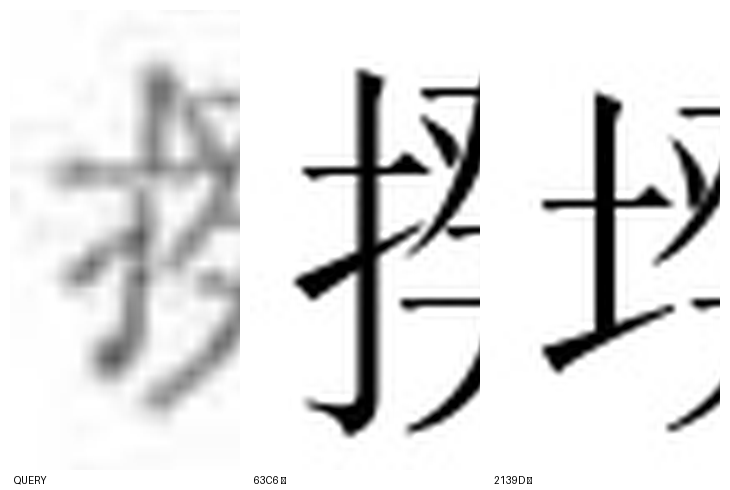
\includegraphics[width=0.46\textwidth]{figs/coix-bo-trai.png}
\hfill
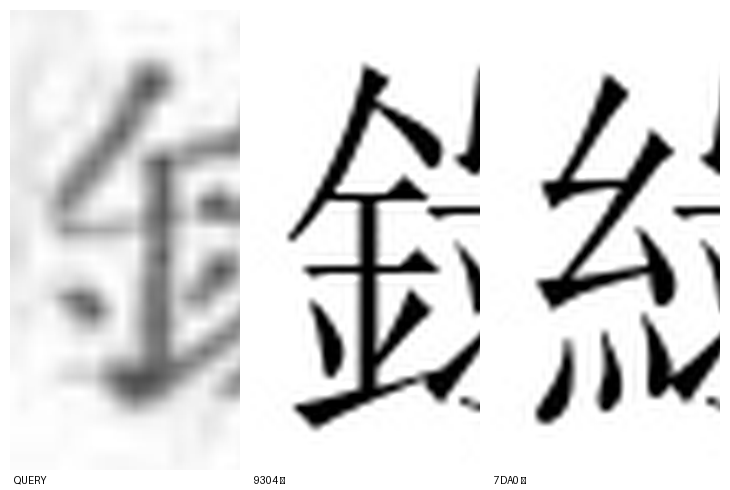
\includegraphics[width=0.46\textwidth]{figs/lujc-bo-trai.png}
\caption{Trái: ``cõi'' --- bộ trái là \nom{土} (nét đáy nằm ngang, sổ dừng ở đó), không phải
\nom{扌} (móc thõng xuống). Nhãn \nom{揆} sai, đúng là \nom{𡎝}. Phải: ``lục'' --- đáy bộ trái là
\emph{một nét ngang} (\nom{金}, tức \nom{錄}), không phải ba chấm của \nom{糸} (\nom{綠}).}
\end{figure}

Kết quả soát: năm dòng lên \code{high}, \code{gia} xuống \code{low}, và \textbf{một nhãn sai}:
\code{coix} từ \nom{揆} sang \nom{𡎝} --- cũng trùng luôn chính tả Kiều ``trong cõi người ta''.

\textbf{Một lỗi gán nhãn duy nhất đã nghiêng kết quả.} Sửa \code{coix} làm embedding \emph{mất} một
ảnh và histogram \emph{được} một ảnh: 29/25 thành 28/26, khoảng cách co từ 4 ảnh xuống 2. Đây là
bằng chứng trực tiếp cho việc bảng trên không chịu nổi sức nặng của một kết luận.

\begin{figure}[h]
\centering
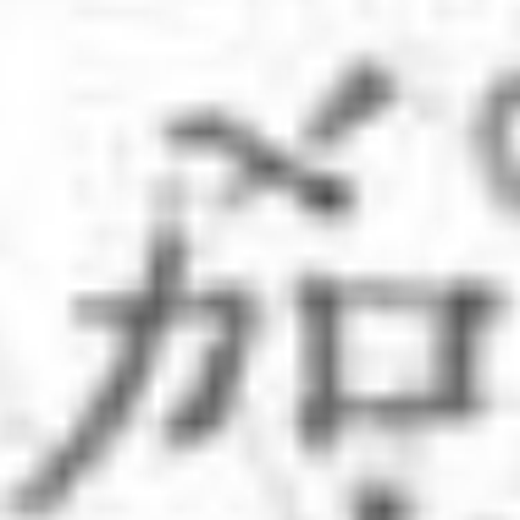
\includegraphics[width=0.30\textwidth]{figs/gia-scan.png}
\caption{Ca \code{gia}. Văn cảnh rất mạnh --- câu ``Rằng năm \textbf{Gia Tĩnh} triều Minh'', niên
hiệu \nom{嘉靖} --- nhưng ảnh \emph{không phải} \nom{嘉}: \nom{嘉} có ba tầng (\nom{士}/\nom{口}/\nom{加}),
ảnh chỉ có hai (một bộ thủ nhỏ trên \nom{加}). Giữa \nom{笳} (\nom{⺮}) và \nom{茄} (\nom{艹}) thì nét
đỉnh đã mờ mất. Để \code{low} và ghi lại cả hai khả năng.}
\end{figure}

Hai dòng \code{trari} và \code{gia} vẫn chưa giải quyết được và \textbf{cần ảnh trang gốc} ---
\code{test\_images/} chỉ có chữ rời, không kèm số câu, nên ``đối chiếu văn cảnh'' ở đây là suy từ
tập từ vựng của mấy câu đầu Kiều chứ không phải tra được đúng vị trí.

\subsection{$n = 59$ là trần cứng của tập test này}

\code{test\_images/} chỉ có 59 ảnh scan và \textbf{không có nguồn scan nào khác trong kho}. Ở
$n = 59$ quanh $p \approx 0{,}5$, khoảng tin cậy 95\% rộng \textbf{$\pm$13,3 điểm}; muốn xuống
$\pm$8 điểm cần $n \approx 150$, xuống $\pm$6 điểm cần $n \approx 300$.

Nghĩa là \textbf{mọi cải tiến dưới $\sim$15 điểm --- gần như chắc chắn bao gồm cả finetune ---
không thể chứng minh trên tập này}. Muốn đo được thì phải có thêm ảnh scan thật, không phải thêm
phương pháp.

% =====================================================================
\section{Có nên thay Faiss \code{IndexFlatIP} bằng chỉ mục xấp xỉ?}

\code{IndexFlatIP} là brute-force chính xác --- $O(N)$ mỗi query --- nên câu hỏi hoàn toàn hợp lý.
Để không nguỵ tạo số, hai loại đo được tách bạch: \textbf{recall} chỉ đo trên embedding thật (vì
recall phụ thuộc phân bố vector), còn \textbf{độ trễ} cho các cỡ chưa có (100k--1M) dùng vector
ngẫu nhiên và được ghi rõ là tổng hợp.

\begin{table}[h]
\centering
\begin{tabular}{llrrrr}
\toprule
chỉ mục & tham số & \code{recall@20} & build & ms/query & nhanh gấp \\
\midrule
\textbf{Flat (exact)} & --- & \textbf{1,0000} & 0,05 s & 0,195 & 1$\times$ \\
HNSW32 & efSearch=64 & 0,9912 & 0,51 s & 0,010 & 20,4$\times$ \\
IVFFlat & nprobe=64 & 0,9843 & 1,90 s & 0,044 & 4,5$\times$ \\
IVFPQ & nprobe=64 & \textbf{0,6047} & 6,16 s & 0,012 & 16,9$\times$ \\
\bottomrule
\end{tabular}
\caption{$N = 26.044$, top-$K$ = 20. HNSW giữ 99,1\% recall mà nhanh gấp 20 lần; IVFPQ nén quá mạnh
cho bài toán này.}
\end{table}

\textbf{Nhưng ở cỡ corpus hiện tại, tăng tốc đó vô nghĩa.} Điểm mấu chốt: embed tăng $O(N)$ còn quét
toàn corpus tăng $O(N^2)$, nên tỉ trọng của search chỉ có tăng. Ở 26k, search chiếm \textbf{6\%}
tổng thời gian --- kể cả tăng tốc vô hạn cũng chỉ rút được 5 giây trên tổng 79 giây. Điểm hoà vốn
nằm quanh $N \approx 300.000$; từ 500k trở đi thì ANN là bắt buộc (ở 1M, exact mất 2,1 giờ mỗi lượt
quét so với $\sim$4,7 phút của HNSW).

\textbf{Khuyến nghị: giữ nguyên \code{IndexFlatIP}} cho tới khi corpus vượt $\sim$300k. Ở giai đoạn
còn đang so sánh chất lượng các backend, nếu search cũng xấp xỉ thì không còn phân biệt được lỗi do
model hay do chỉ mục.

% =====================================================================
\section{Hạ tầng dữ liệu cho finetune}

Corpus có \textbf{đúng 1 ảnh cho 1 ký tự} (26.044 ảnh / 26.044 ký tự). Metric learning cần
\emph{cặp dương}, nên hiện tại \textbf{không tồn tại cặp nào} để dạy mô hình bỏ qua khác biệt kiểu
chữ. Mỗi ký tự đã có mã Unicode nên render lại qua nhiều font là cách rẻ nhất để có cặp dương.

Bảy nhóm font, độ phủ đo bằng bảng \code{cmap} của từng font (\emph{không đoán} --- ký tự không có
trong \code{cmap} bị bỏ qua thay vì render ra ô tofu, thứ sẽ đầu độc cặp dương). Hợp nhất:
\textbf{26.033/26.044 = 100,0\%}, trung bình 5,05 kiểu chữ/ký tự, tổng \textbf{131.604 ảnh render}
cộng 26.044 ảnh corpus = 157.648 view trên 26.044 lớp.

\subsection{Tập này có chạm đúng chỗ hỏng không?}

Lấy 400 ảnh render mỗi font làm query, tìm trên index corpus 26k:

\begin{center}
\begin{tabular}{lrr}
\toprule
query & \code{hit@1} & \code{hit@10} \\
\midrule
\code{babelstone} & 0,7800 & 0,9500 \\
\code{hanamin} & 0,7200 & 0,9350 \\
\textbf{\code{lxgw-kai}} (khải thư) & \textbf{0,6350} & 0,8775 \\
\textbf{trung bình} ($n$=2.800) & \textbf{0,7018} & \textbf{0,9214} \\
\emph{scan thật} & \emph{0,0847} & \emph{0,1864} \\
\bottomrule
\end{tabular}
\end{center}

Font khó nhất (\code{lxgw-kai}) cũng là font gần chất bút lông nhất --- thứ tự khó dễ đi đúng theo
hướng cần. Nhưng độ khó của nó \textbf{kém xa} thực tế: 0,6350 so với 0,0847, chênh gần 9 lần.
\textbf{Render đa font là điều kiện cần, chưa phải điều kiện đủ.}

\subsection{Suy giảm ảnh cho giống scan}

Đo trực tiếp 59 ảnh scan so với ảnh render cho thấy khoảng cách lớn nhất là \emph{độ nét}
($15{,}6$ so với $102{,}2$, lệch 6,55$\times$), rồi tới tương phản (2,54$\times$) và nhiễu.
\code{scan\_augment.degrade()} mô phỏng sáu trục đó theo đúng thứ tự vật lý của một trang scan, và
khoảng tham số được \textbf{hiệu chỉnh theo số đo} chứ không chỉnh mò: sai lệch log trung bình
$0{,}880 \to 0{,}103$, tốt hơn 8,5 lần, cả sáu chỉ số về trong khoảng 0,77--1,00$\times$ so với scan
thật.

\begin{center}
\begin{tabular}{lrr}
\toprule
\code{strength} & \code{hit@1} & \code{hit@10} \\
\midrule
0,0 (render sạch) & 0,7018 & 0,9214 \\
0,4 & 0,4179 & 0,6832 \\
0,7 & 0,2825 & 0,5239 \\
\textbf{1,0} & \textbf{0,1986} & \textbf{0,4161} \\
\emph{scan thật} & \emph{0,0847} & \emph{0,1864} \\
\bottomrule
\end{tabular}
\end{center}

Augmentation cũ chỉ đạt 0,6732 --- dễ hơn scan thật 9,4 lần. Bản mới ở \code{strength} 1,0 đạt
0,1986, \textbf{dễ hơn 2,8 lần}. Phần còn lại 2,8$\times$ \emph{không} lấp được bằng xử lý ảnh: mọi
phép trong \code{degrade()} là \emph{nhiễu ảnh}, còn scan thật khác ở chỗ chữ được viết bằng bút
lông theo lối hành thư --- nét nối liền, tỉ lệ bộ phận xê dịch, có nét bị lược. Đó là khác biệt
\textbf{cấu trúc}. Muốn lấp nốt phải có chữ bút lông thật (MCCD: 329.715 ảnh, 7.765 lớp, 10 thể
chữ) hoặc scan Hán-Nôm thật (NomNaOCR / IHR-NomDB).

% =====================================================================
\section{Hạn chế}

\begin{itemize}
  \item Các chỉ số ở mục 4--6 là \textbf{proxy}, không phải đánh giá của người. Mức đồng thuận giữa
        các backend chỉ 7,6--12,9\%, nên đánh giá bằng người là việc \emph{chặn} mọi kết luận khác.
  \item \textbf{$n = 59$ là quá nhỏ, và đó là toàn bộ dữ liệu scan hiện có.} Mọi so sánh ở mục về
        chuẩn hoá hình học đều nằm trong khoảng nhiễu.
  \item Nhãn Phần 2 do \textbf{so hình} mà ra, không phải do chuyên gia Hán-Nôm đọc. Sau vòng soát
        lại còn 6/59 dòng \code{med}/\code{low}, và vòng soát đó đã sửa một nhãn sai làm khoảng cách
        embedding--histogram co từ 4 ảnh xuống 2.
  \item Ảnh trong \code{test\_images/} là chữ viết tay/hành thư còn corpus là khải thư in --- mọi số
        ở mục~\ref{sec:that} đo trên đúng một cặp phân phối này.
  \item Oracle IDS-Jaccard dựa trên \code{SHAPE\_MORPH}, vốn chỉ có ở 96,9\% ký tự và bản thân cũng
        là nhãn do người biên soạn.
  \item Recall của ANN chỉ đo ở $N = 26.044$; recall của HNSW thường giảm khi $N$ tăng, nên con số
        99,1\% không được suy diễn cho mốc 1M.
\end{itemize}

% =====================================================================
\section{Kết luận}

\begin{enumerate}
  \item \textbf{Chuyển sang \code{chinese-clip-large}.} Hơn baseline ResNet18 2,31 lần ở
        \code{radical@k} và 2,05 lần ở \code{ids\_jaccard@k}, với chi phí GPU chấp nhận được.
  \item \textbf{Không scale tiếp.} ViT-H \emph{kém hơn} ViT-L 4,0\% --- large là điểm ngọt.
  \item \textbf{Lỗi \code{conv1} không phải nguyên nhân}, và đây là kết quả âm có giá trị: nó biện
        minh cho việc đổi hẳn kiến trúc thay vì vá baseline.
  \item \textbf{\code{radical@k} = 0,5 không phải bão hoà.} Trần thực tế là 0,7338 chứ không phải
        0,9862, nên mô hình đang ở 73\% quãng đường và 24,4$\times$ mức ngẫu nhiên.
  \item \textbf{Giữ nguyên \code{IndexFlatIP}} --- search chỉ chiếm 6\% thời gian; điểm hoà vốn của
        ANN nằm quanh $N \approx 300.000$.
  \item \textbf{Phần 2 nên dùng \code{--method embedding}} --- nhưng lý do là \emph{chất lượng điểm
        số} (64/64 so với 62/64 ở phép thử tự truy hồi; histogram nén cả nhóm vào dải 0,003), không
        phải accuracy. Trên scan thật hai bên chỉ chênh 2 ảnh trên 59.
  \item \textbf{Trên ảnh query thật, hiệu năng thấp hơn nhiều so với proxy gợi ý} ---
        \code{hit@1} = 0,0847. Nguyên nhân chính là khoảng cách thư pháp, không phải model kém.
  \item \textbf{Phần 2 mới là chỗ dùng được ngay}: 0,4746, gấp 2,4 lần chọn ngẫu nhiên trong nhóm.
\end{enumerate}

\subsection*{Việc tiếp theo, xếp theo thứ tự}

\begin{enumerate}
  \item \textbf{Scan thêm ảnh thật.} Đây là nút thắt hiện tại: ở $n = 59$ không có cải tiến nào dưới
        15 điểm chứng minh được. Cần $n \approx 150$ để xuống $\pm$8 điểm.
  \item \textbf{Đánh giá bằng người} trên $\sim$200 cặp, để biết \code{radical@k} lệch bao nhiêu so
        với ``trông giống''.
  \item \textbf{Ensemble} \code{chinese-clip-large} + \code{dinov2} --- hai model chỉ trùng 12,9\%
        top-$k$ và mạnh ở hai chỉ số khác nhau, chưa cần huấn luyện gì.
  \item \textbf{Finetune} metric learning trên thành phần IDS, huấn luyện với cặp dương từ
        \code{render\_fonts.py --augment N --strength 1.0}, held-out chia \emph{theo bộ thủ}.
\end{enumerate}

% =====================================================================
\appendix
\section{Tái lập số liệu}

Mọi số trong báo cáo tái lập được bằng các lệnh sau, chạy từ trong thư mục dự án:

\begin{quote}\small\ttfamily
\# thêm --dtype fp16 cho chinese-clip-large và chinese-clip-huge\\
.venv/bin/python search\_all\_chars\_in\_corpus.py --backend <backend> --device cuda\\
.venv/bin/python benchmark\_extractors.py\\
.venv/bin/python benchmark\_search.py\\
.venv/bin/python analyze\_metric\_ceiling.py\\[4pt]
\# đánh giá trên ảnh query thật\\
.venv/bin/python evaluate\_test\_images.py --device cuda\\
.venv/bin/python evaluate\_test\_images.py --device cuda --normalize query\\
.venv/bin/python evaluate\_test\_images.py --sheets\\
.venv/bin/python evaluate\_test\_images.py --part 2 \textbackslash\\
\hspace*{2em}--labels output/label\_sheets/label\_template.csv\\
.venv/bin/python evaluate\_test\_images.py --part 2 \textbackslash\\
\hspace*{2em}--labels output/label\_sheets/label\_template.csv --min-confidence high\\[4pt]
\# hạ tầng dữ liệu cho finetune\\
bash download\_fonts.sh\\
.venv/bin/python render\_fonts.py\\
.venv/bin/python scan\_augment.py --calibrate\\
.venv/bin/python render\_fonts.py --augment 2 --strength 1.0
\end{quote}

\section{File kết quả}

\begin{center}
\small
\begin{tabular}{ll}
\toprule
file & nội dung \\
\midrule
\code{output/benchmark\_summary.xlsx} & 3 sheet: \code{Metrics}, \code{Agreement}, \code{Samples} \\
\code{output/benchmark\_search.xlsx} & so exact với ANN \\
\code{output/contact\_sheet\_<backend>.png} & query (khung đỏ) + 5 lân cận đầu \\
\code{output/output\_top\_k\_similar\_char\_<backend>.xlsx} & top-20 đầy đủ cho toàn corpus \\
\code{output/embeddings\_<backend>.npz} & cache embedding \\
\code{output/label\_sheets/*.png} + \code{label\_template.csv} & phiếu gán nhãn Phần 2 \\
\code{output/rendered/<font>/<UNICODE>.png} & 131.604 ảnh render đa font \\
\bottomrule
\end{tabular}
\end{center}

\end{document}
